% This is LLNCS.DEM the demonstration file of
% the LaTeX macro package from Springer-Verlag
% for Lecture Notes in Computer Science,
% version 2.4 for LaTeX2e as of 16. April 2010
%
\documentclass[a4paper,fontsize=11pt]{scrartcl}



% Anpassungen an DC Template
\usepackage[a4paper, left=2.9cm,right=2.87cm,bottom=3cm,top=3cm,headsep=1.27cm]{geometry}
\setlength{\parskip}{0.5em}
\renewcommand{\tablename}{TABLE} 
\renewcommand{\figurename}{FIG.} 
\usepackage{titlesec}
\titlespacing\section{0pt}{12pt plus 2pt minus 2pt}{6pt plus 1pt minus 1pt}
\titlespacing\subsection{0pt}{12pt plus 2pt minus 2pt}{3pt plus 1pt minus 1pt}
\addtokomafont{title}{\fontsize{14pt}{1em}\selectfont}
\setkomafont{section}{\fontsize{12pt}{0pt}\selectfont}
\addtokomafont{subsection}{\fontsize{11pt}{0pt}\selectfont}
% \addtokomafont{author}{\fontsize{12pt}{1em}\selectfont}
\usepackage{scrpage2}
\clearscrheadfoot
\pagestyle{scrheadings}
\renewcommand*{\titlepagestyle}{scrheadings}
\chead{\fontsize{9pt}{0pt}\selectfont Proc. Int'l Conf. on Dublin Core and Metadata Applications 2015}
\usepackage{apacite}


\date{}

\usepackage[utf8]{inputenc}

% URL handling
\usepackage{url}
\urlstyle{same}

% Todos
\usepackage[colorinlistoftodos]{todonotes}
\newcommand{\ke}[1]{\todo[size=\small, color=orange!40]{\textbf{Kai:} #1}}
\newcommand{\tb}[1]{\todo[size=\small, color=green!40]{\textbf{Thomas:} #1}}


% \usepackage{makeidx}  % allows for indexgeneration -- yes, but we don't need this

\usepackage{amsmath}

% monospace within text
\newcommand{\ms}[1]{\texttt{#1}}

% examples
\usepackage{fancyvrb}
\DefineVerbatimEnvironment{ex}{Verbatim}{numbers=left,numbersep=2mm,frame=single,fontsize=\scriptsize}

\usepackage{xspace}
% Einfache und doppelte Anfuehrungszeichen
\newcommand{\qs}{``} 
\newcommand{\qe}{''\xspace} 
\newcommand{\sqs}{`} 
\newcommand{\sqe}{'\xspace} 

% checkmark
\usepackage{tikz}
\def\checkmark{\tikz\fill[scale=0.4](0,.35) -- (.25,0) -- (1,.7) -- (.25,.15) -- cycle;} 

% Xs
\usepackage{pifont}

% Tabellenabstände kleiner
\setlength{\intextsep}{10pt} % Vertical space above & below [h] floats
\setlength{\textfloatsep}{10pt} % Vertical space below (above) [t] ([b]) floats
% \setlength{\abovecaptionskip}{0pt}
% \setlength{\belowcaptionskip}{0pt}

\usepackage{tabularx}
\newcommand{\hr}{\hline\noalign{\smallskip}} % für die horizontalen linien in tabellen

\newenvironment{DL}{
  %\scriptsize
  %\sffamily
  \vspace{0cm}
	\begin{center}
  \begin{tabular}{r l}

}{
  \end{tabular}
	\end{center}
}

% just makes the table prettier (see \toprule, \bottomrule, etc. commands below)
\usepackage{booktabs}

% Tabellenabstände kleiner
\setlength{\intextsep}{10pt} % Vertical space above & below [h] floats
\setlength{\textfloatsep}{10pt} % Vertical space below (above) [t] ([b]) floats
% \setlength{\abovecaptionskip}{0pt}
% \setlength{\belowcaptionskip}{0pt}

\usepackage{tabularx}

\usepackage{float}

\begin{document}

\title{\vspace{-1em}Guidance, please! Towards a framework for RDF-based constraint languages.}

\author{Thomas Bosch\\GESIS – Leibniz Institute \\for the Social Sciences, Germany\\thomas.bosch@gesis.org \and Kai Eckert\\Stuttgart Media University, Germany\\eckert@hdm-stuttgart.de}

\maketitle
\vspace{-3em}
\section*{Abstract}
In the context of the DCMI RDF Application Profile task group and the W3C Data Shapes Working Group solutions for the proper formulation of constraints and validation of RDF data on these constraints are developed. Several approaches and constraint languages exist but there is no clear favorite and none of the languages is able to meet all requirements raised by data practitioners.
To support the work, a comprehensive, community-driven database has been created where case studies, use cases, requirements and solutions are collected. Based on this database,
we published by today 81 types of constraints that are required by various stakeholders for data applications. We generally use this collection of constraint types to gain a better understanding of the expressiveness of existing solutions and gaps that still need to be filled. 
Regarding the implementation of constraint languages, we already proposed to use high-level languages to describe the constraints, but map them to SPARQL queries in order to execute the actual validation; we demonstrated this approach for Description Set Profiles.
In this paper, we generalize from the experience of implementing Description Set Profiles by introducing an abstraction layer that is able to describe any constraint type in a way that is more or less straight-forwardly transformable to SPARQL queries. 
It provides a basic terminology and classification system for RDF constraints to foster discussions on RDF validation.
We demonstrate that using another layer on top of SPARQL helps to implement validation consistently accross constraint languages and simplifies the actual implementation of new languages.

%When using the developed vocabulary to intermediately represent constraints,
%depending on the individual type of constraint one or multiple particular constraining elements are applied.
%We base these constraining elements on formal logic.
%As constraints of 2/3 of all constraint types are expressible by logical constructs from description logics,
%we may use logical constructs as constraining elements.
%In order to be able to support all constraint types, however,
%we determined for each constraint type more intuitive constraining elements in natural language like \emph{conditional properties}, \emph{allowed values}, and \emph{language tag minimum cardinality}.
%A title is required for books.
%This constraint of the constraint type \emph{required properties (R-68)} can be either expressed by the existential quantifier $\exists$ from description logics or more intuitively using the constraining element \emph{required properties}.

%As SPARQL is generally seen as the method of choice to validate data according to certain constraints and
%as RDF data can be validated on constraints of any constraint type by means of SPARQL,
%we use SPIN, a SPARQL-based way to validate RDF data, as implementation language 
%to actually execute the validation of RDF data.
%Thereby, constraints may either be 
%(1) expressed by domain specific constraint languages like OWL 2 and DSP or
%(2) represented by the proposed vocabulary. 

%The majority of these constraint types can be expressed in description logics which provides their logical underpinning.
%In this paper, we provide a basic terminology and classification system for RDF constraints.\tb{The contributions of this paper are the following. (1)...}
%We developed a vocabulary to describe constraints of any RDF constraint type generically. 
%%(whether expressible in description logics or not).
%We show how to transform constraints, expressed by any constraint language \ms{$\alpha$}, into generically expressed constraints and into constraints represented by any other constraint language \ms{$\beta$} and discuss why these transformations are useful.
%We explain how to overcome the necessity to implement the validation of each constraint type for multiple constraint languages by providing mappings to generically expressed constraints.

%The main contributions of this paper are:
%(1) We provide a basic terminology and classification system for RDF constraints to lay the ground for discussions on RDF validation.
%(2) As current high-level constraint languages do not support all constraint types, 
%we developed a vocabulary to describe constraints of any constraint type in a generic way and specified its underlying semantics.
%(3) We show how to enhance the interoperability of constraints expressed by different languages by using the proposed vocabulary 
%to intermediately represent constraints 
%%as an intermediate generic representation 
%which enables transformations between semantically equivalent constraints.
%(4) We explain how constraint languages may reuse validation implementations which are provided once for each constraint type.

\hspace{-1.4em}
\textbf{Keywords:}
RDF validation; RDF constraints; RDF constraint types, RDF validation requirements; Linked Data; Semantic Web

\section{Introduction}
%The purpose of OWL 2 ontologies is to perform reasoning on RDF data and not to validate RDF data conforming to these ontologies.
%OWL 2 is based on the {\em non-unique name assumption} (nUNA) whereas RDF validation requires that different names represent different objects ({\em unique name assumption} (UNA)). 
%Reasoning in OWL 2 is based on the semantics of {\em open-world assumption} (OWA), i.e., a statement cannot be inferred to be false if it cannot be proved to be true  which fits its primary design purpose: to represent knowledge on the World Wide Web. 
%On the other hand, many RDF validation scenarios require the {\em closed-world assumption} (CWA) (i.e., a statement is inferred to be false if it cannot be proved to be true).
%This ambiguity in semantics is one of the main reasons why OWL 2 has not been adopted as a standard constraint language for RDF validation.  
%For this reason, we cannot use OWL 2 ontologies for RDF validation as we use XML Schemas, DTDs, RELAX NG, or Schematron to validate XML documents.

The proper validation of RDF data according to constraints is a common requirement of data practitioners. 
Among the reasons for the success of XML is the possibility to formulate fine-grained constraints to be met by the data and to validate the data according to these constraints using powerful systems like \emph{DTD}, \emph{XML Schema}, \emph{RELAX NG}, or \emph{Schematron}.

In 2013, the \emph{W3C} organized the \emph{RDF Validation Workshop}\footnote{\url{http://www.w3.org/2012/12/rdf-val/}}
where experts from industry, government, and academia discussed first RDF validation use cases. 
%for RDF data validation and constraint formulation.
In 2014, two working groups on RDF validation have been established: 
the \emph{W3C RDF Data Shapes Working Group}\footnote{\url{http://www.w3.org/2014/rds/charter}} and the \emph{DCMI RDF Application Profiles Task Group}\footnote{\url{http://wiki.dublincore.org/index.php/RDF-Application-Profiles}}. 
We collected the findings of these working groups and initiated a database of RDF validation requirements\footnote{Online available at \url{http://purl.org/net/rdf-validation}}
with the intention to collaboratively collect case studies, use cases, requirements, and solutions in a comprehensive and structured way \cite{BoschEckert2014}. 
Based on our work in the \emph{DCMI} and in cooperation with the \emph{W3C} working group,
we identified by today 81 constraint types, where each type corresponds to a specific requirement in the database. In a technical report, we explain each constraint type in detail and give examples for each represented by different constraint languages \cite{BoschNolleAcarEckert2015}.

Various constraint languages exist or are being developed that support more or less of these constraint types. For our work, we focus on the following four as the ones that are most popular among data practitioners, often mentioned on mailing lists and/or being candidates or prototypes for the upcoming W3C recommendation:
\emph{Description Set Profiles (DSP)}, \emph{Resource Shapes (ReSh)}, \emph{Shape Expressions (ShEx)}, and the \emph{Web Ontology Language} \emph{(OWL)}. Despite the fact that OWL is arguably not a constraint language, it is widely used in practice as such under the closed-world and unique name assumptions.

With its direct support of validation via \emph{SPARQL}, the \emph{SPARQL Inferencing Notation (SPIN)} is also very popular to formulate and check constraints \cite{Fuerber2010}. We consider SPIN as a low-level language in contrast to the other constraint languages where specific language constructs exist to define constraints in a declarative and in comparison more intuitive way -- although SPARQL aficionados might object particularly to the latter point.

The power of SPIN is shown in 
Table \ref{tab:constraint-type-specific-expressivity}, where we list the fraction (and absolute numbers in brackets) of how many constraint types each of these languages supports \cite{BoschNolleAcarEckert2015}. 
We further see that OWL 2 is currently the most expressive high-level constraint language, at least according to the pure number of constraint types supported. This does not preclude that other constraint languages are better suited for certain applications, either because they support some types that are not supported by OWL or because the constraint representation is more appealing to the data practitioners -- producers as well as consumers who again might have different needs and preferences.

\begin{table}
	\centering
	  %\caption{Constraint Type Specific Expressivity}
		\caption{Constraint Type Specific Expressivity of Constraint Languages}
	  \scriptsize
		\begin{tabular}{c|c|c|c|c}
      %\textbf{Expressivity Class} & $Expr(\overline{\mathcal{CT}_R})$ (42) & $Expr(\mathcal{CT}_R)$ (32) \\		
			\emph{DSP} & \emph{ReSh} & \emph{ShEx} & OWL 2 & \emph{SPIN} \\	
      \hline
			17.3 (14) & 25.9 (21) & 29.6 (24) & 67.9 (55) & \textbf{100.0} \textbf{(81)} 
		\end{tabular}
	\label{tab:constraint-type-specific-expressivity}
\end{table}

We formerly demonstrated that a high-level constraint language, Description Set Profiles, can be implemented by mapping the language to SPIN using SPARQL CONSTRUCT queries \cite{BoschEckert2014-2}. We provide a validation environment where own mappings from arbitrary constraint languages can be provided and tested.\footnote{Available at \url{http://purl.org/net/rdfval-demo}, source code available at: \url{https://github.com/boschthomas/rdf-validator}.}

The creation of such mappings is in many cases not straight-forward and requires profound knowledge of SPARQL, as the following example demonstrates:

The constraint type \emph{minimum qualified cardinality restrictions} which corresponds to the requirement \emph{R-75}\footnote{Requirements are identified in the database by an R and a number, additionally an alphanumeric identifier is provided, in this case R-75-MINIMUM-QUALIFIED-CARDINALITY-ON-PROPERTIES. Online at: \url{http://lelystad.informatik.uni-mannheim.de/rdf-validation/?q=node/82}} can be used to formulate the constraint
that \emph{publications} must have at least one \emph{author} which must be a \emph{person}.

This constraint can be expressed as follows using different constraint languages:

\begin{ex}[commandchars=\\\{\}]
\textit{OWL 2:} Publication a owl:Restriction ;
          owl:minQualifiedCardinality 1 ;
          owl:onProperty author ;
          owl:onClass Person .
		
\textit{ShEx:} Publication \{ author @Person\{1, \} \}

\textit{ReSh:} Publication a rs:ResourceShape ; rs:property [
          rs:propertyDefinition author ;
          rs:valueShape Person ;
          rs:occurs rs:One-or-many ; ] .
		
\textit{DSP:} [ dsp:resourceClass Publication ; dsp:statementTemplate [ 
          dsp:minOccur 1 ; dsp:maxOccur "infinity" ; 
          dsp:property author ; 
          dsp:nonLiteralConstraint [ dsp:valueClass Person ] ] ] .
					
\textit{SPIN:} CONSTRUCT \{ [ a spin:ConstraintViolation ... . ] \} WHERE \{ 
          ?this ?p ?o ; a ?C .
          BIND ( \textit{qualifiedCardinality}( ?this, ?p, ?C ) AS ?c ) .
          BIND( STRDT ( STR ( ?c ), xsd:nonNegativeInteger ) AS ?cardinality ) .
          FILTER ( ?cardinality < 1 ) . 
          FILTER ( ?C = Person ) .
          FILTER ( ?p = author ) . \}
						
\textit{SPIN function qualifiedCardinality:}										
SELECT ( COUNT ( ?arg1 ) AS ?c ) WHERE \{ ?arg1 ?arg2 ?o . ?o a ?arg3 . \}
\end{ex}

Note that the SPIN representation is NOT a mapping, but a direct expression of the constraint using a SPARQL CONSTRUCT query that creates a spin:ConstraintViolation if the constraint is violated. The mapping for DSP is much more complicated and can be found in the mappings provided by us.\footnote{Online: \url{https://github.com/boschthomas/rdf-validation/blob/b6a275fb5d71a92ae33d3b6aadd5f447351214b7/SPIN/DSP_SPIN-Mapping.ttl#L4665}}

On the other hand, it can be seen that the higher-level constraint languages are comparatively similar, there seems to be a pattern, a common way to express this type of constraint. Therefore, a mapping from a high-level language to another high-level language would be considerably easier. Unfortunately, there is not (yet) a high-level language that supports all constraint types. 

In this paper, we build on the experience gained from mapping several constraint languages to SPIN and from the analysis of the identified constraint types to create an intermediate layer, a framework that is able to describe the mechanics of all constraint types and that can be used to map high-level languages more easily. 



\section{Motivation}

Even with an upcoming W3C recommendation, it can be expected that several constraint languages will be used in practice in future -- consider the situation in the XML world, where a standardized schema language was available from the beginning and yet additional ways to formulate and check constraints have been created. Therefore, 
semantically equivalent \emph{specific constraints} represented in different languages will exist.
This raises two questions: 
\begin{enumerate}
 \item How can we ensure that two semantically equivalent constraints are actually validated consistently?
 \item How can we support the transformation of semantically equivalent constraints from one contraint language to another?
\end{enumerate}



\paragraph{Consistent implementation.}
Even though SPIN provides a convenient way to represent constraints and to validate data according to these constraints, the implementation of a high-level constraint language still requires a tedious mapping to SPIN with a certain degree of freedom as to how a constraint violation is actually represented and how exactly the violation of the contraint is checked.
Our framework therefore proides a common ground that is solely based on the abstract definitions of the constraint types, as identified in our database. By providing a \emph{SPIN} mapping
for each constraint type\footnote{RDF-CV to SPIN online available at: \url{https://github.com/boschthomas/RDF-CV-2-SPIN}\label{RDF-CV-2-SPIN}}, it is ensured that the details of the SPIN implementation are consistent irrespective of the constraint language and that the validation leads always to exactly the same results.  


\paragraph{Constraint transformation.} Consistent implementations of constraint languages provide some advantage, but it could be argued that they are not important enough to justify the additional layer. The situation, however, is different when transformations from one constraint language to another are desired, i.e., to transform a \emph{specific constraint} (\emph{$sc_{\alpha}$}) of any constraint type expressed by language \emph{$\alpha$} into a semantically equivalent \emph{specific constraint} (\emph{$sc_{\beta}$}) of the same constraint type represented by any other language \emph{$\beta$}.
By defining mappings between equivalent \emph{specific constraints} and the corresponding \emph{generic constraint} (\emph{gc}) we are able to convert them automatically: 
\begin{align*}
  gc &=  m_1(sc_{\alpha}) \\
  sc_{\beta} &= m_2'(gc) 
\end{align*}

Thereby, we do not need to define mappings for each constraint type and each possible combination of constraint languages. Assuming that we are able to express a single constraint type like \emph{minimum qualified cardinality restrictions} within 10 languages, $n \cdot n-1 = 90$ mappings would be needed -- as mapping generally are not invertible. 
With an intermediate generic representation of constraints, on the other side, we only need to define for each constraint type $2n = 20$ mappings -- where $10$ mappings should already exist if we have an implementation in our framework. 
To summarize, if language developers are willing to provide two mappings -- forward and backward -- to our framework for each supported constraint type, we not only would get the consistent implementation of all languages, it would also be possible to transform semantically equivalent constraints into all constraint languages.


\section{Towards a framework} 
\label{sec:vocabulary}

When we implemented DSP and other constraint languages using SPARQL as intermediate language \cite{BoschEckert2014-2}, we found that many mappings actually resemble each other; particularly the mappings of the same constraint type in different languages, but also the mappings of different constraint types, though the latter only on a very superficial, structural level. The basic idea of our framework is very simple: we aim at reducing the representation of constraint types to the absolute minimum that has to be provided in a mapping to generate the appropriate SPIN implementation. Consider again our example from above for the SPIN implementation of \emph{minimum qualified cardinality restrictions}:

\begin{ex}[commandchars=\\\{\}]
\textit{SPIN:} CONSTRUCT \{ [ a spin:ConstraintViolation ... . ] \} WHERE \{ 
          ?this ?p ?o ; a ?C .
          BIND ( \textit{qualifiedCardinality}( ?this, ?p, ?C ) AS ?c ) .
          BIND( STRDT ( STR ( ?c ), xsd:nonNegativeInteger ) AS ?cardinality ) .
          FILTER ( ?cardinality < 1 ) . 
          FILTER ( ?C = Person ) .
          FILTER ( ?p = author ) . \}
						
\textit{SPIN function qualifiedCardinality:}										
SELECT ( COUNT ( ?arg1 ) AS ?c ) WHERE \{ ?arg1 ?arg2 ?o . ?o a ?arg3 . \}
\end{ex}

However this SPIN code looks like, all we have to provide to make it work is the desired minimum cardinality (?cardinality), the property to be constrained (?p) and the class for which this property should be constrained (?C). All other variables are bound internally. So we could reduce the effort of the mapping by simply providing these three values, which are readily available in all representations of this constraint type:

\begin{ex}[commandchars=\\\{\}]
\textit{OWL 2:} Publication a owl:Restriction ;
          owl:minQualifiedCardinality 1 ;
          owl:onProperty author ;
          owl:onClass Person .
		
\textit{ShEx:} Publication \{ author @Person\{1, \} \}

\textit{ReSh:} Publication a rs:ResourceShape ; rs:property [
          rs:propertyDefinition author ;
          rs:valueShape Person ;
          rs:occurs rs:One-or-many ; ] .
		
\textit{DSP:} [ dsp:resourceClass Publication ; dsp:statementTemplate [ 
          dsp:minOccur 1 ; dsp:maxOccur "infinity" ; 
          dsp:property author ; 
          dsp:nonLiteralConstraint [ dsp:valueClass Person ] ] ] .
\end{ex}

In further investigation of all kind of constraints and particularly the list of constraint types, we aimed at identifying the building blocks of such constraints to come up with a concise representation of every constraint type. 


\subsection{Building blocks}

At the core, we use a very simple conceptual model for constraints, using a small vocabulary called \emph{RDF Constraints Vocabulary (RDF-CV)}\footnote{Online available at: \url{https://github.com/boschthomas/RDF-Constraints-Vocabulary}}. The conceptual model is shown in Figure \ref{fig:RDF-CV-conceptual-model}.
\begin{figure}[H]
	\centering
		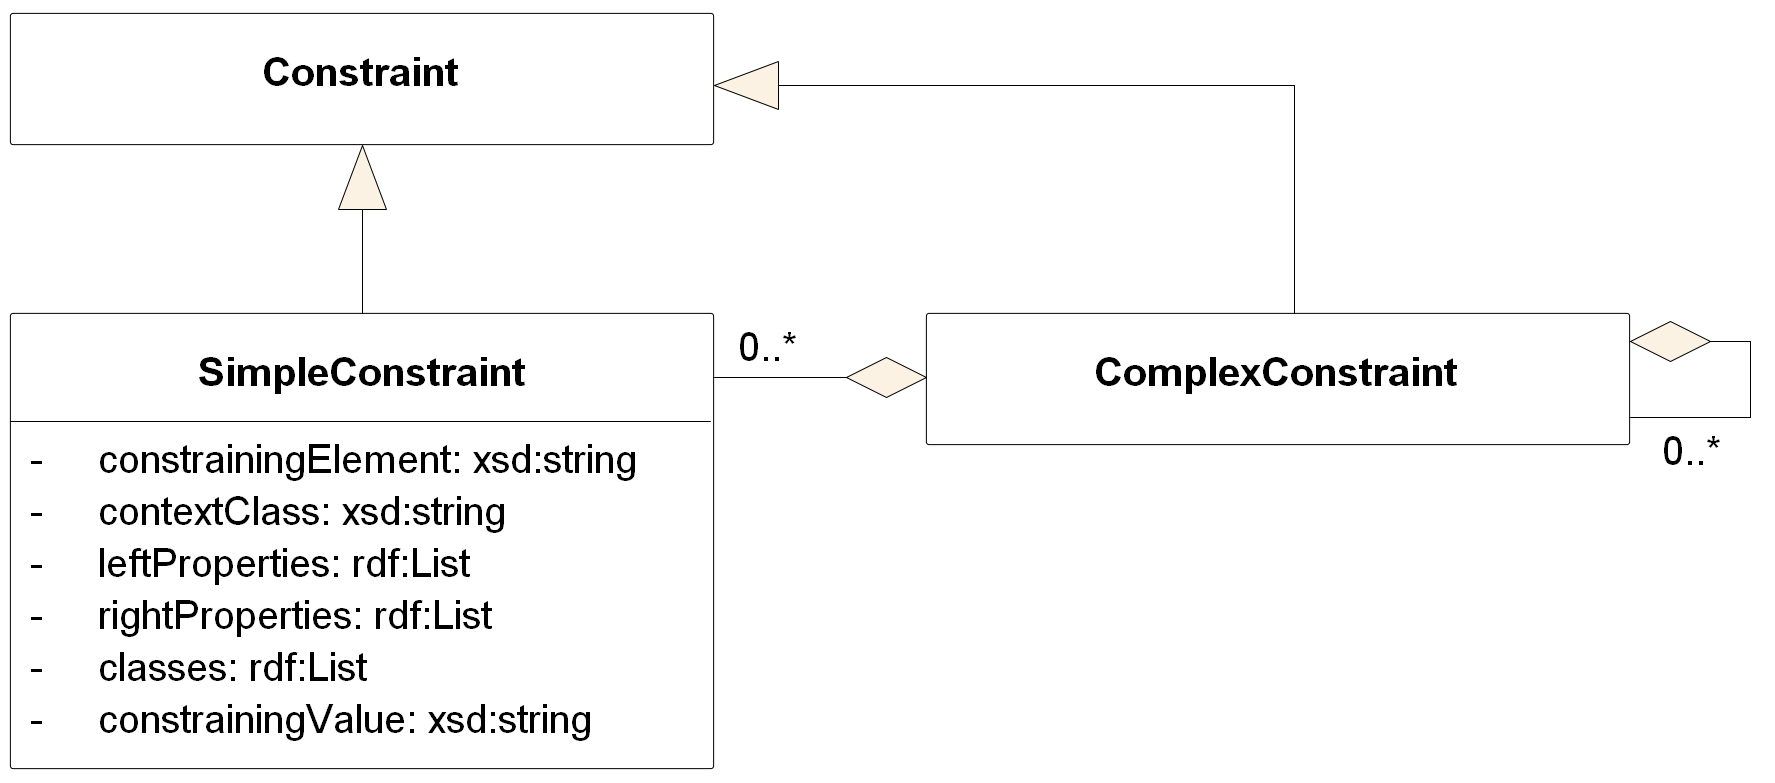
\includegraphics[width=0.60\textwidth]{images/RDF-CV.png}
	\caption{\emph{RDF Constraints Vocabulary (RDF-CV)} Conceptual Model}
	\label{fig:RDF-CV-conceptual-model}
\end{figure}

\emph{Simple constraints} denotes the set of atomic constraints with respect to a single constraining element -- we will come to the notion of a constraining element in a second. In contrast, there are  
\emph{complex constraints}, i.e., the set of constraints which are created out of \emph{simple} and/or other \emph{complex constraints}. This structure therefore allows to build complex constraints out of other (simple or complex) constraints. Regarding our database of constraint types, 60\% of the constraint types are simple constraints and 26\% are complex constraints. 
Constraints of additional 14\% of the constraint types are \emph{complex constraints} as well which can be simplified and therefore formulated as \emph{simple constraints} if additional constraining elements are introduced to cover them.

The properties describing a simple constrained are very structural. The central property is the \emph{constraining element} which refers to one of 103 contraining elements described in our technical report \cite{BoschNolleAcarEckert2015}. Constraining elements are for example taken from Description Logics, another concrete example would be 'regex' where a regular expression is checked against some property value. Sometimes the constraining elements directly correspond to a constraint type, sometime (as for regex) they are shared by several constraint types. Complex constraints again need several constraing elements to be expressed.

Irrespective of and additonal to the constraining element, there are properties to describe the actual constraint, they can also be seen as parameters for the constraining element. The \emph{context class} limits the constraint to individuals of a specific class. Depending on the constraining elements, a list of \emph{classes} can be provided, for example to determine the valid classes for a value or to define a class intersection to be used in a constraint. \emph{leftProperties} and \emph{rightProperties} are lists usually containing properties the constraint is applied to. A typical example for a constraint with a right hand side list of properties would be R43, literal value comparision, where constraints like birthDate $<$ deathDate can be expressed.

Finally, the \emph{constrainig value} contains a literal value to be checked against; for instance in the case of the 'regex' element, it contains the regular expression to be evaluated.

This simple structure plus the constraining elements form the building blocks of our proposed framework. In the technical report \cite{BoschNolleAcarEckert2015}, we list for every constraint type its representation in our framework which not only shows that constraints of any constraint type can indeed be described generically in this way, but which also forms the starting point for any mappings using this framework.

\paragraph{Formal approach and semantics.}

A cornerstone of the framework is the generic representation of a constraint, which can often be done using \emph{Description Logics (DL)}, as for the \emph{minimum qualified cardinality restrictions}: {\small\ms{Publication $\sqsubseteq$ $\geq$1 author.Person}}

It turned out that 64\% of the 81 constraint types are actually expressible in DL. Only for the remaining 36\%, other means, i.e., other constraining elements, had to be identified. This is not surprising if we consider that OWL is based on Description Logics. When we talk about using Description Logics to represent constraints, we have to establish once more that the semantics of OWL and Description Logics differ from the semantics of constraint languages regarding the open world assumption (OWA) and the non-unique naming assumption (nUNA). Both are usually assumed when dealing with OWL or DL, whereas validation usually assumes a closed world (CWA) and unique naming (UNA), i.e., if a desired property is missing, this leads to a violation and if two resources are named differently, they are assumed to be different resources. 

We won't get into details about these assumptions here, but it has to be noted that the applied semantics have to be defined if validation is performed, as the results would differ under different semantics. Precisely, we found that for 56.8\% of the constraint types validation results differ if the CWA or the OWA is assumed 
and for 66.6\% of the constraint types validation results are different in case the UNA or the nUNA is assumed \cite{BoschNolleAcarEckert2015}.

For the purpose of a consistent implementation and transformation of constraints, constraints are semantically equivalent  
if they detect the same set of violations regardless of RDF data, 
which means whenever the constraints are applied to any RDF data they point out the same violations.


\subsection{\emph{Simple Constraints}}


The \emph{minimum qualified cardinality restriction (R-75)} {\small\ms{Publication $\sqsubseteq$ $\geq$1 author.Person,}}
which restricts publications to have at least one author which must be a person,
is an example of a property constraint on \emph{author}
which holds for all individuals of the class \emph{Publication}.
Table \ref{tab:property-constraint-cardinality-restriction} displays how the property constraint is generically represented using the RDF-CV.
\begin{table}[H]
  \scriptsize
  \sffamily
  \vspace{0cm}
	\caption{Minimum Qualified Cardinality Restriction as Property Constraint}
	\label{tab:property-constraint-cardinality-restriction}
	\centering
		\begin{tabular}{c|c|c|c|c|c|c}
      \textbf{constraint set} & \textbf{context class} & \textbf{left property list} & \textbf{right p. list} & \textbf{classes} & \textbf{constraining element} & \textbf{c. value} \\
      \hline
      property & Publication & author & - & Person & $\geq$ & 1 \\
		\end{tabular}
\end{table}

%The \emph{constraining element} indicates the actual type of constraint like DL concept and role constructors ($\sqsubseteq$, $\equiv$, $\sqcap$, $\sqcup$, $\neg$, $\exists$, $\forall$, $\geq$, $\leq$), (in)equality (=, $\ne$), and further keywords for constraint types whose constraints cannot be expressed in DL (e.g., regular expressions and constraining facets). 

The \emph{constraining element} is an intuitive term which indicates the actual type of constraint. For the majority of the constraint types, there is exactly one constraining element. For the constraint type \emph{property domain (R-25, R-26)} whose constraints restrict domains of properties, e.g., there is only one constraining element with exactly the same identifier \emph{property domain}. For a few constraint types, however, one constraining element is not sufficient to describe all possible constraints of a particular constraint type and therefore multiple constraining elements may be stated. The constraint type \emph{language tag cardinality (R-48, R-49)}, for instance, is used to restrict data properties to have a minimum, maximum, or exact number of relationships to literals with selected language tags. Thus, three constraining elements are needed to express each possible constraint of that constraint type.

If constraint types are expressible in DL, associated constraining elements are formally based on DL constructs like concept and role constructors ($\sqsubseteq$, $\equiv$, $\sqcap$, $\sqcup$, $\neg$, $\exists$, $\forall$, $\geq$, $\leq$), equality (=), and inequality ($\ne$). In case constraint types cannot be expressed in DL such as \emph{data property facets (R-46)} or \emph{literal pattern matching (R-44)}, we reuse widely known terms from SPARQL (e.g., \emph{regex}) or XML Schema (e.g., \emph{minInclusive}) as constraining elements. For some constraint types like \emph{minimum qualified cardinality restrictions (R-75)}, it is more intuitive and concise to directly apply DL constructs like the \emph{at-least restriction} ($\geq$) as constraining elements. We provide a complete list of all constraining elements which can be used to express constraints of any constraint type \cite{BoschNolleAcarEckert2015}. 

In some cases, a constraint is only complete when a \emph{constraining value} is stated in addition to the constraining element
and simple constraints may refer to a list of \emph{classes}. The constraining element of the property constraint {\small\ms{Publication $\sqsubseteq$ $\geq$1 author.Person},} e.g., is \emph{$\geq$}, the constraining value is \emph{1}, and the list of classes includes the class \emph{Person} which restricts the objects of the property \emph{author} to be persons.

For property constraints, \emph{left} and \emph{right property lists} are specified.
The assignment of properties to these lists happens relative to the constraining element.
\emph{Object Property Paths} (\emph{R-55})
ensure that if an individual \emph{x} is connected by a sequence of object properties with an individual \emph{y}, 
then \emph{x} is also related to \emph{y} by a particular object property. 
As \emph{Stephen-Hawking} is the author of the book \emph{A-Brief-History-Of-Time} 
%{\small\ms{(authorOf(Stephen-Hawking, A-Brief-History-Of-Time))}} 
whose genre is \emph{Popular-Science}, 
%{\small\ms{(genre(A-Brief-History-Of-Time, Popular-Science)),}}
the object property path {\small\ms{authorOf $\circ$ genre $\sqsubseteq$ authorOfGenre}} infers that \emph{Stephen-Hawking} is an author of the genre \emph{Popular-Science}. 
%{\small\ms{(authorOfGenre(Stephen-Hawking, Popular-Science))}.}
Thus, when representing the property constraint using the RDF-CV (see Table \ref{tab:property-constraint-object-property-paths}), the properties \emph{authorOf} and \emph{genre} are placed on the left side of the constraining element \emph{property paths}
and the property \emph{authorOfGenre} on its right side. As this property constraint holds for all individuals within the data, the context class is set to the \emph{DL top concept} $\top$ which stands for the super-class of all possible classes.
\begin{table}[H]
  \scriptsize
  \sffamily
  \vspace{0cm}
	\caption{Object Property Paths as Property Constraint}
	\label{tab:property-constraint-object-property-paths}
	\centering
		\begin{tabular}{l|l|l|l|l|l|l}
      \textbf{c. set} & \textbf{context class} & \textbf{left p. list} & \textbf{right p. list} & \textbf{classes} & \textbf{c. element} & \textbf{c. value} \\
      \hline
      property & $\top$ & authorOf, genre & authorOfGenre & $\top$ & property paths & - \\
		\end{tabular}
\end{table}

There are simple constraints which are not expressible in DL but can still be described using the RDF-CV such as constraints of the type \emph{literal pattern matching} (\emph{R-44}) which restrict literals to match given patterns. The \emph{universal quantification (R-91)} {\small\ms{Book $\sqsubseteq$ $\forall$ identifier.ISBN}} ensures that books can only have valid \emph{ISBN} identifiers, i.e., strings that match a given regular expression.
%Even though, the restriction of the datatype \emph{ISBN} cannot be expressed in DL, \emph{OWL 2 DL} can be used to express the \emph{literal pattern matching} constraint:
%\begin{ex}
%ISBN a RDFS:Datatype ; owl:equivalentClass [ a RDFS:Datatype ;
    %owl:onDatatype xsd:string ; 
    %owl:withRestrictions ([ xsd:pattern "^\d{9}[\d|X]" ])] .
%\end{ex} 
%The first OWL 2 axiom explicitly declares {\em ISBN} to be a datatype. %\er{Why start from second and then first? Also better we say "owl axiom" when we talk axiom of owl, to prevent ambiguity.}\tb{resolved}
%The second OWL 2 axiom defines {\em ISBN} as an abbreviation for a datatype restriction on {\em xsd:string}. 
%The datatype {\em ISBN} can be used just like any other datatype like in the \emph{universal restriction} above.
%There are multiple use cases associated with the requirement to match literals according to given patterns (\emph{Literal Pattern Matching}\footnote{Corresponds to \emph{R-44-PATTERN-MATCHING-ON-RDF-LITERALS}}).
%The enterprise vessel, e.g.,  can only have the registry numbers "NCC-1701", "NCC-1701-A", "NCC-1701-B", "NCC-1701-C", "NCC-1701-D", or "NCC-1701-E".
%The universal restriction can be represented in DL:
%\ms{Enterprise $\sqsubseteq$ $\forall$ registryNumber.RegistryNumber}.
%The restriction of the datatype \ms{RegistryNumber}, however, cannot be expressed in DL, but OWL 2 DL can be used anyway to express the literal pattern matching constraint:
%
%\begin{ex}
%RegistryNumber
    %a rdfs:Datatype ; owl:equivalentClass [ a rdfs:Datatype ;
        %owl:onDatatype xsd:string ;
        %owl:withRestrictions ( [ xsd:pattern "NCC-1701([-][A-E])?" ] ) ] .
%\end{ex}
%The second axiom defines \ms{RegistryNumber} as an abbreviation for a datatype restriction on \ms{xsd:string}. 
%The first axiom explicitly declares \ms{RegistryNumber} to be a datatype. 
%The datatype \ms{RegistryNumber} can be used just like any other datatype like in the universal restriction above.
%The \emph{literal pattern matching} constraint validates \emph{ISBN} literals according to the regular expression causing constraint violations for triples which do not not match. 
%\ms{Janeway commandsEnterprise Voyager} and \ms{Voyager registryNumber "NCC-74656"\textasciicircum{}\textasciicircum{}RegistryNumber}, 
%but not for the triples \ms{Picard commandsEnterprise Enterprise} and \ms{Enterprise registryNumber "NCC-1701-E"\textasciicircum{}\textasciicircum{}RegistryNumber}.

Even though, constraints of the type \emph{literal pattern matching} cannot be expressed in DL, OWL 2 can be used to formulate the constraint:

\begin{ex}
ISBN a RDFS:Datatype ; owl:equivalentClass [ a RDFS:Datatype ;
    owl:onDatatype xsd:string ; 
    owl:withRestrictions ([ xsd:pattern "^\d{9}[\d|X]$" ])] .
\end{ex}\$$

The first OWL 2 axiom explicitly declares {\em ISBN} to be a datatype. %\er{Why start from second and then first? Also better we say "owl axiom" when we talk axiom of owl, to prevent ambiguity.}\tb{resolved}
The second OWL 2 axiom defines {\em ISBN} as an abbreviation for a datatype restriction on \emph{xsd:string}. 
The datatype {\em ISBN} can be used just like any other datatype like in the universal quantification above.

Table \ref{tab:simple-constraint-not-expressible-in-dl)} presents (1) in the first line how the literal pattern matching simple constraint which is not expressible in DL and (2) in the second line how the universal quantification complex constraint which is expressible in DL are represented using the RDF-CV. Thereby, the context class \emph{ISBN}, whose instances must satisfy the simple constraint, is reused within the list of classes the complex constraint refers to. The literal pattern matching constraint type introduces the constraining element \emph{regex} whose validation has to be implemented once like for any other constraining element.
%In general, validation has to be implemented once for each \emph{generic constraint type} which is not expressible in DL. 
%\begin{gcotable}
%property & Enterprise & registryNumber & - & RegistryNumber & $\forall$ & - \\
%class & RegistryNumber & - & - & xsd:string & regex & 'NCC-1701([-][A-E])?' \\
%\end{gcotable}
\begin{table}[H]
  \scriptsize
  \sffamily
  \vspace{0cm}
	\caption{Simple Constraints which are not Expressible in DL}
	\label{tab:simple-constraint-not-expressible-in-dl)}
	\centering
		\begin{tabular}{l|l|l|l|l|l|l}
      \textbf{c. set} & \textbf{context class} & \textbf{left p. list} & \textbf{right p. list} & \textbf{classes} & \textbf{c. element} & \textbf{c. value} \\
      \hline
      class & ISBN & - & - & xsd:string & regex & '\string^\text{$\backslash$d$\{9\}$[$\backslash$d$\mid$X]}\$' \\
      property & Book & identifier & - & ISBN & universal quantification & - \\
		\end{tabular}
\end{table} %\tb{Erman, can you please format the regular expression in the table above correctly?}

\subsection{\emph{Complex Constraints}}

%\emph{Complex constraints} are composed out of \emph{simple constraints} and/or \emph{complex constraints}.
Complex constraints of the constraint type \emph{context-specific exclusive or of property groups} (\emph{R-13}) restrict individuals of given classes to have all properties of exactly one of multiple mutually exclusive property groups. Publications, e.g., are either identified by an \emph{ISBN} and a title (for books) or by an \emph{ISSN} and a title (for periodical publications), but it should not be possible to assign both identifiers to a given publication. This complex constraint is expressible in \emph{ShEx}: 

\begin{ex}
Publication { 
    ( isbn string , title string ) |
    ( issn string , title string ) }
\end{ex}

As \emph{The-Great-Gatsby} is a publication with an \emph{ISBN} and a title without an \emph{ISSN}, \emph{The-Great-Gatsby} is considered as a valid publication. This complex constraint is generically expressible in DL:
%This \emph{complex constraint} is expressible specifically by \emph{ShEx} and generically by DL (and can therefore be mapped to the \emph{RDF-CV} \cite{BoschEckert2015-2}).

%Half-Klingons, e.g., either have a klingon mother and a human father or a human mother and a klingon father, which can be expressed by ShEx:

%\begin{ex}
%Half-Klingon { 
    %( klingonMother Klingon , humanFather Human ) |
    %( humanMother Human , klingonFather Klingon ) }
%\end{ex}

%\begin{ex}[commandchars=\\\{\}]
%\textit{ShEx:} Publication { ( isbn string , title string ) | ( issn string , title string ) }
%\end{ex}

%As \ms{B'Elanna Torres} is a \ms{Half-Klingon} with a klingon mother and a human father, the following data is valid:

%\begin{ex}
%BElannaTorres a Half-Klingon ;
    %klingonMother Miral ; humanFather JohnTorres .
%\end{ex}

%\begin{DL}
%rdf:type(BElannaTorres,Half-Klingon) \\
%klingonMother(BElannaTorres,Miral) \\
%klingonMother(BElannaTorres,JohnTorres)
%\end{DL}
%The \emph{complex constraint} is mapped to the \emph{RDF-CV} (see Table \ref{tab:complex-constraints}) and expressed in DL as follows:

%\begin{DL}
%Half-Klingon $\sqsubseteq$ ($\neg$E $\sqcap$ F) $\sqcup$ (E $\sqcap$ $\neg$F) \\ 
%E $\equiv$ A $\sqcap$ B \\
%F $\equiv$ C $\sqcap$ D \\
%A $\sqsubseteq$ $\geq$ 1 klingonMother.Klingon $\sqcap$ $\leq$ 1 klingonMother.Klingon \\
%B $\sqsubseteq$ $\geq$ 1 humanFather.Human $\sqcap$ $\leq$ 1 humanFather.Human \\
%C $\sqsubseteq$ $\geq$ 1 humanMother.Human $\sqcap$ $\leq$ 1 humanMother.Human \\
%D $\sqsubseteq$ $\geq$ 1 klingonFather.Klingon $\sqcap$ $\leq$ 1 klingonFather.Klingon \\
%\end{DL}

\begin{DL}
\textbf{Publication $\sqsubseteq$ ($\neg$E $\sqcap$ F) $\sqcup$ (E $\sqcap$ $\neg$F)} , E $\equiv$ A $\sqcap$ B , F $\equiv$ C $\sqcap$ D \\
A $\sqsubseteq$ $\geq$ 1 isbn.string $\sqcap$ $\leq$ 1 isbn.string , B $\sqsubseteq$ $\geq$ 1 title.string $\sqcap$ $\leq$ 1 title.string \\
C $\sqsubseteq$ $\geq$ 1 issn.string $\sqcap$ $\leq$ 1 issn.string , D $\sqsubseteq$ $\geq$ 1 title.string $\sqcap$ $\leq$ 1 title.string \\
\end{DL}

%\begin{gcotable}
%class & Half-Klingon & - & - & $\neg$E $\sqcap$ F, E $\sqcap$ $\neg$F & $\sqcup$ & - \\
%class & $\neg$E $\sqcap$ F & - & - & $\neg$E, F & $\sqcap$ & - \\
%class & E $\sqcap$ $\neg$F & - & - & E, $\neg$F & $\sqcap$ & - \\
%class & $\neg$E & - & - & E & $\neg$ & - \\
%class & E & - & - & A, B & $\sqcap$ & - \\
%class & $\neg$F & - & - & F & $\neg$ & - \\
%class & F & - & - & C, D & $\sqcap$ & - \\
%class & A & - & - & A1, A2 & $\sqcap$ & - \\
%property & A1 & klingonMother & - & Klingon & $\geq$ & 1 \\
%property & A2 & klingonMother & - & Klingon & $\leq$ & 1 \\
%class & B & - & - & B1, B2 & $\sqcap$ & - \\
%property & B1 & humanFather & - & Human & $\geq$ & 1 \\
%property & B2 & humanFather & - & Human & $\leq$ & 1 \\
%class & C & - & - & C1, C2 & $\sqcap$ & - \\
%property & C1 & humanMother & - & Human & $\geq$ & 1 \\
%property & C2 & humanMother & - & Human & $\leq$ & 1 \\
%class & D & - & - & D1, D2 & $\sqcap$ & - \\
%property & D1 & klingonFather & - & Klingon & $\geq$ & 1 \\
%property & D2 & klingonFather & - & Klingon & $\leq$ & 1 \\
%\end{gcotable}

%\begin{table}[H]
  %\scriptsize
  %\sffamily
  %\vspace{0cm}
	%\caption{Complex Constraints}
	%\label{tab:complex-constraints}
	%\centering
		%\begin{tabular}{l|l|l|l|l|l|l}
      %\textbf{c. set} & \textbf{context class} & \textbf{left p. list} & \textbf{right p. list} & \textbf{classes} & \textbf{c. element} & \textbf{c. value} \\
      %\hline
%class & Publication & - & - & $\neg$E $\sqcap$ F, E $\sqcap$ $\neg$F & $\sqcup$ & - \\
%class & $\neg$E $\sqcap$ F & - & - & $\neg$E, F & $\sqcap$ & - \\
%class & E $\sqcap$ $\neg$F & - & - & E, $\neg$F & $\sqcap$ & - \\
%class & $\neg$E & - & - & E & $\neg$ & - \\
%class & E & - & - & A, B & $\sqcap$ & - \\
%class & $\neg$F & - & - & F & $\neg$ & - \\
%class & F & - & - & C, D & $\sqcap$ & - \\
%class & A & - & - & A1, A2 & $\sqcap$ & - \\
%property & A1 & isbn & - & string & $\geq$ & 1 \\
%property & A2 & isbn & - & string & $\leq$ & 1 \\
%class & B & - & - & B1, B2 & $\sqcap$ & - \\
%property & B1 & title & - & string & $\geq$ & 1 \\
%property & B2 & title & - & string & $\leq$ & 1 \\
%class & C & - & - & C1, C2 & $\sqcap$ & - \\
%property & C1 & issn & - & string & $\geq$ & 1 \\
%property & C2 & issn & - & string & $\leq$ & 1 \\
%class & D & - & - & D1, D2 & $\sqcap$ & - \\
%property & D1 & title & - & string & $\geq$ & 1 \\
%property & D2 & title & - & string & $\leq$ & 1 \\
		%\end{tabular}
%\end{table}

%Even though, tools may generate \emph{generic constraints} automatically, this 
The DL statements demonstrate that the complex constraint is composed of many other complex constraints (\emph{minimum (R-75) and maximum qualified cardinality restrictions (R-76)}) and simple constraints (\emph{intersection (R-15/16)}, \emph{disjunction (R-17/18)}, and \emph{negation (R-19/20)}). Constraints of almost 14\% of the constraint types are complex constraints which can be simplified and therefore formulated as simple constraints when using them in terms of syntactic sugar. As \emph{exact (un)qualified cardinality restrictions (=n)} and \emph{exclusive or (XOR) of property groups} are frequently used complex constraints, we propose to simplify them in form of simple constraints. As a consequence, the \emph{context-specific exclusive or of property groups (R-13)} complex constraint is represented as a generic constraint by means of the RDF-CV more intuitively and concisely (see Table \ref{tab:simplified-complex-constraints}).

%\begin{gcotable}
%class & Half-Klingon & - & - & E, F & XOR \\
%class & E & - & - & A, B & $\sqcap$ \\
%class & F & - & - & C, D & $\sqcap$ \\
%property & A & klingonMother & - & Klingon & = & 1 \\
%property & B & humanFather & - & Human & = & 1 \\
%property & C & humanMother & - & Human & = & 1 \\
%property & D & klingonFather & - & Klingon & = & 1 \\
%\end{gcotable}

\begin{table}[H]
  \scriptsize
  \sffamily
  \vspace{0cm}
	\caption{Simplified Complex Constraints}
	\label{tab:simplified-complex-constraints}
	\centering
		\begin{tabular}{l|l|l|l|l|l|l}
      \textbf{c. set} & \textbf{context class} & \textbf{left p. list} & \textbf{right p. list} & \textbf{classes} & \textbf{c. element} & \textbf{c. value} \\
      \hline
class & Publication & - & - & E, F & XOR of property groups & - \\
class & E & - & - & A, B & intersection & - \\
class & F & - & - & C, D & intersection & - \\
property & A & isbn & - & string & = & 1 \\
property & B & title & - & string & = & 1 \\
property & C & issn & - & string & = & 1 \\
property & D & title & - & string & = & 1 \\
		\end{tabular}
\end{table}

%\emph{Complex constraints} can be simplified and therefore formulated as \emph{simple constraints} when using them in terms of syntactic sugar.
%There are three forms of \emph{OWL RBox axioms}: \emph{role inclusions}, \emph{equivalence} and \emph{disjointness}. 
%\emph{OWL} provides a variety of other axiom types: \emph{role transitivity}, \emph{symmetry}, \emph{asymmetry}, \emph{reflexivity} and \emph{irreflexivity}. 
%These axiom types are sometimes considered as basic axiom types in DL - using some suggestive notation such as
%\ms{Trans(ancestorOf)} to express that the role \emph{ancestorOf} is transitive.
%Such axioms, however, are just syntactic sugar - 
%all role characteristics can be expressed using the basic features of DL.
%
%The \emph{irreflexive object properties} constraint type (\emph{R-60}) 
%restricts that no individual is connected by a given object property to itself \cite{Kroetzsch2012}.
%With the following \emph{irreflexive object property} constraint, for instance, one can state that individuals cannot be authors of themselves:
%\begin{DL}
%\ms{$\top$ $\sqsubseteq$ $\neg$ $\exists authorOf.Self$}
%\end{DL}
%When mapped to the \emph{RDF-CV} (see Table \ref{tab:irreflexive-object-properties-as-complex-constraints}), the \emph{complex constraint} aggregates three \emph{simple constraints} (one \emph{property} and two \emph{class constraints}):
%
%%\begin{gcotable}
%%property & $\exists$ marriedTo . Self & marriedTo & - & Self & $\exists$ & - \\
%%class & $\neg$ $\exists$ marriedTo . Self & - & - & $\exists$ marriedTo . Self & $\neg$ & - \\
%%class & $\top$ & - & - & $\top$, $\neg$ $\exists$ marriedTo . Self & $\sqsubseteq$ & - \\
%%\end{gcotable}
%
%\begin{table}[H]
  %\scriptsize
  %\sffamily
  %\vspace{0cm}
	%\caption{Irreflexive Object Properties as Complex Constraints}
	%\label{tab:irreflexive-object-properties-as-complex-constraints}
	%\centering
		%\begin{tabular}{l|l|l|l|l|l|l}
      %\textbf{c. set} & \textbf{context class} & \textbf{left p. list} & \textbf{right p. list} & \textbf{classes} & \textbf{c. element} & \textbf{c. value} \\
      %\hline
%property & $\exists$ authorOf.Self & marriedTo & - & Self & $\exists$ & - \\
%class & $\neg$ $\exists$ authorOf.Self & - & - & $\exists$ authorOf.Self & $\neg$ & - \\
%class & $\top$ & - & - & $\top$, $\neg$ $\exists$ authorOf.Self & $\sqsubseteq$ & - \\
		%\end{tabular}
%\end{table}
%
%When using the \emph{OWL RBox axiom} \emph{role irreflexivity} in terms of syntactic sugar, 
%the \emph{complex constraint} can be expressed more concisely in form of a \emph{simple property constraint} with exactly the same semantics (see Table \ref{tab:irreflexive-object-properties-as-simple-constraints}):
%
%%\begin{gcotable}
%%property & $\top$ & marriedTo & - & - & irreflexive & - \\
%%\end{gcotable}
%
%\begin{table}[H]
  %\scriptsize
  %\sffamily
  %\vspace{0cm}
	%\caption{Irreflexive Object Properties as Simple Constraints}
	%\label{tab:irreflexive-object-properties-as-simple-constraints}
	%\centering
		%\begin{tabular}{l|l|l|l|l|l|l}
      %\textbf{c. set} & \textbf{context class} & \textbf{left p. list} & \textbf{right p. list} & \textbf{classes} & \textbf{c. element} & \textbf{c. value} \\
      %\hline
%property & $\top$ & authorOf & - & - & irreflexive & - \\
		%\end{tabular}
%\end{table}
The \emph{primary key properties (R-226)} constraint type is often useful to declare a given (datatype) property as the primary key of a class, so that a system can enforce uniqueness. 
Books, e.g., are uniquely identified by their \emph{ISBN}, i.e., the property \emph{isbn} is inverse functional \ms{$(\ms{funct } isbn\sp{\overline{\ }})$}
which can be represented using the RDF-CV in form of a complex constraint consisting of two simple constraints (see Table \ref{tab:primary-key-properties-as-complex-constraints}).

%\begin{gcotable}
%property & $\top$ & commandAuthorizationCode$^{-}$ & commandAuthorizationCode$^{-}$ & - & inverse & - \\
%property & $\top$ & commandAuthorizationCode$^{-}$ & - & - & functional & - \\
%\end{gcotable}

\begin{table}[H]
  \scriptsize
  \sffamily
  \vspace{0cm}
	\caption{Primary Key Properties as Complex Constraints}
	\label{tab:primary-key-properties-as-complex-constraints}
	\centering
		\begin{tabular}{l|l|l|l|l|l|l}
      \textbf{c. set} & \textbf{context class} & \textbf{left p. list} & \textbf{right p. list} & \textbf{classes} & \textbf{c. element} & \textbf{c. value} \\
      \hline
property & $\top$ & isbn$^{-}$ & isbn$^{-}$ & - & inverse property & - \\
property & Book & isbn$^{-}$ & - & - & functional property & - \\
		\end{tabular}
\end{table}

Keys, however, are even more general, i.e., a generalization of inverse functional properties \cite{Schneider2009}.
A key can be a datatype, an object property, or a chain of properties.
For these generalization purposes, as there are different sorts of keys, and as keys can lead to undecidability, 
DL is extended with a special construct \emph{keyfor} \cite{Lutz2005}.
When using keyfor (\ms{isbn keyfor Book}), 
the complex constraint can be simplified and thus formulated as a simple constraint which looks like the following in concrete RDF turtle syntax:

%\begin{gcotable}
%property & StarFleetOfficer & commandAuthorizationCode & - & - & keyfor & - \\
%\end{gcotable}

%\begin{table}[H]
  %\scriptsize
  %\sffamily
  %\vspace{0cm}
	%\caption{Primary Key Properties as Simple Constraints}
	%\label{tab:primary-key-properties-as-simple-constraints}
	%\centering
		%\begin{tabular}{l|l|l|l|l|l|l}
      %\textbf{c. set} & \textbf{context class} & \textbf{left p. list} & \textbf{right p. list} & \textbf{classes} & \textbf{c. element} & \textbf{c. value} \\
      %\hline
%property & Book & isbn & - & - & keyfor & - \\
		%\end{tabular}
%\end{table}

\begin{ex}[commandchars=\\\{\}]
[   a \textit{rdfcv:PropertyConstraint} , \textit{rdfcv:SimpleConstraint} ;
    \textit{rdfcv:contextClass} Book ; \textit{rdfcv:leftProperties} ( isbn ) ; \textit{rdfcv:constrainingElement} "keyfor" ] .
\end{ex}

Complex constraints of frequently used constraint types which correspond to DL axioms like \emph{transitivity}, \emph{symmetry}, \emph{asymmetry}, \emph{reflexivity} and \emph{irreflexivity} can also be simplified in form of simple constraints. Although, these DL axioms are expressible by basic DL features, they can also be used in terms of syntactic sugar \cite{BoschEckert2015-2}.

Constraints of the \emph{irreflexive object properties (R-60)} constraint type ensure that no individual is connected by a given object property to itself \cite{Kroetzsch2012}. With the irreflexive object property constraint {\small\ms{$\top$ $\sqsubseteq$ $\neg$ $\exists authorOf.Self$}}, e.g., one can state that individuals cannot be authors of themselves. When represented using the RDF-CV, the complex constraint aggregates three simple constraints - one property and two class constraints (see Table \ref{tab:irreflexive-object-properties-as-complex-constraints}).

%\begin{gcotable}
%property & $\exists$ marriedTo . Self & marriedTo & - & Self & $\exists$ & - \\
%class & $\neg$ $\exists$ marriedTo . Self & - & - & $\exists$ marriedTo . Self & $\neg$ & - \\
%class & $\top$ & - & - & $\top$, $\neg$ $\exists$ marriedTo . Self & $\sqsubseteq$ & - \\
%\end{gcotable}

\begin{table}[H]
  \scriptsize
  \sffamily
  \vspace{0cm}
	\caption{Irreflexive Object Properties as Complex Constraints}
	\label{tab:irreflexive-object-properties-as-complex-constraints}
	\centering
		\begin{tabular}{l|l|l|l|l|l|l}
      \textbf{c. type} & \textbf{context class} & \textbf{left p. list} & \textbf{right p. list} & \textbf{classes} & \textbf{c. element} & \textbf{c. value} \\
      \hline
property & $\exists$ authorOf.Self & authorOf & - & Self & existential quantification & - \\
class & $\neg$ $\exists$ authorOf.Self & - & - & $\exists$ authorOf.Self & negation & - \\
class & $\top$ & - & - & $\top$, $\neg$ $\exists$ authorOf.Self & sub-class & - \\
		\end{tabular}
\end{table}

When using the irreflexive object property constraint in terms of syntactic sugar, 
the complex constraint can be expressed more concisely in form of a simple property constraint with exactly the same semantics (see Table \ref{tab:irreflexive-object-properties-as-simple-constraints}):

%\begin{gcotable}
%property & $\top$ & marriedTo & - & - & irreflexive & - \\
%\end{gcotable}

\begin{table}[H]
  \scriptsize
  \sffamily
  \vspace{0cm}
	\caption{Irreflexive Object Properties as Simple Constraints}
	\label{tab:irreflexive-object-properties-as-simple-constraints}
	\centering
		\begin{tabular}{l|l|l|l|l|l|l}
      \textbf{c. type} & \textbf{context class} & \textbf{left p. list} & \textbf{right p. list} & \textbf{classes} & \textbf{c. element} & \textbf{c. value} \\
      \hline
property & $\top$ & authorOf & - & - & irreflexive property & - \\
		\end{tabular}
\end{table}

%Starfleet officers, e.g., are uniquely identified by their command authorization code (e.g. to activate and cancel auto-destruct sequences).
%It means that the property \emph{commandAuthorizationCode} is inverse functional - mapped to DL and the \emph{RDF-CV} as follows:
%
%\begin{DL}
%$(\ms{funct } commandAuthorizationCode\sp{\overline{\ }})$
%\end{DL}
%
%%\begin{gcotable}
%%property & $\top$ & commandAuthorizationCode$^{-}$ & commandAuthorizationCode$^{-}$ & - & inverse & - \\
%%property & $\top$ & commandAuthorizationCode$^{-}$ & - & - & functional & - \\
%%\end{gcotable}
%
%\begin{table}
  %\scriptsize
  %\sffamily
  %\vspace{0cm}
	%\centering
		%\begin{tabular}{l|l|l|l|l|l|l}
      %\textbf{c. type} & \textbf{context class} & \textbf{left p. list} & \textbf{right p. list} & \textbf{classes} & \textbf{c. element} & \textbf{c. value} \\
      %\hline
%property & $\top$ & commandAuthorizationCode$^{-}$ & commandAuthorizationCode$^{-}$ & - & inverse & - \\
%property & $\top$ & commandAuthorizationCode$^{-}$ & - & - & functional & - \\
		%\end{tabular}
	%\caption{Primary Key Properties as Complex Constraints}
	%\label{tab:primary-key-properties-as-complex-constraints}
%\end{table}
%
%Keys, however, are even more general, i.e., a generalization of inverse functional properties \cite{Schneider2009}.
%A key can be a datatype property, an object property, or a chain of properties.
%For this generalization purposes, as there are different sorts of key, and as keys can lead to undecidability, 
%DL is extended with \emph{key boxes} and a special \emph{keyfor} construct\cite{Lutz2005}.
%This leads to the following DL and \emph{RDF-CV} mappings (only one \emph{simple property constraint}):
%
%\begin{DL}
%commandAuthorizationCode \ms{keyfor} StarfleetOfficer
%\end{DL}

%\begin{table}
  %\scriptsize
  %\sffamily
  %\vspace{0cm}
	%\centering
		%\begin{tabular}{l|l|l|l|l|l|l}
      %\textbf{c. type} & \textbf{context class} & \textbf{left p. list} & \textbf{right p. list} & \textbf{classes} & \textbf{c. element} & \textbf{c. value} \\
      %\hline
%property & StarFleetOfficer & commandAuthorizationCode & - & - & keyfor & - \\
		%\end{tabular}
	%\caption{Primary Key Properties as Simple Constraints}
	%\label{tab:primary-key-properties-as-simple-constraints}
%\end{table}

%\begin{itemize}
  %\item domain and range
	%\item Primary Key Properties
	%\item ( Exact Qualified Cardinality Restrictions on Properties )
%\end{itemize}

%\subsection{Disjoint Classes}
%
%\begin{DL}
%Hologram $\sqcap$ Human $\sqsubseteq$ $\perp$\\
%Alternative:\\
%$Hologram \sqsubseteq \neg Human$
%\end{DL}
%
%\subsection{Minimum Qualified Cardinality Restrictions on Properties}
%
%\begin{DL}
%$FederationCaptain \sqsubseteq Federation \sqcap \geq1 commandsVessel . Vessel $
%\end{DL}

%\section{Transformations and Automatic Validation of Specific Constraints}
%\section{Transformations between Specific Constraints (Expressed by Different Constraint Languages)}
%\section{Transformations between Specific Constraints}

%\section{Validation of Specific and Generic Constraints}

\subsection{Constraint Transformation}

Constraint of the type \emph{minimum qualified cardinality restriction (R-75)} expressed in OWL 2:

\begin{ex}[commandchars=\\\{\}]
Publication 
    a owl:Restriction ;
    owl:minQualifiedCardinality 1 ;
    owl:onProperty author ;
    owl:onClass Person .
\end{ex}

The same constraint expressed generically using the RDF-CV:

\begin{ex}[commandchars=\\\{\}]
[   a rdfcv:SimpleConstraint ;
    rdfcv:contextClass :Publication ;
    rdfcv:leftProperties ( :author ) ;
    rdfcv:classes ( :Person ) ;
    rdfcv:constrainingElement "minimum qualified cardinality restriction" ;
    rdfcv:constrainingValue 1 ] .
\end{ex}

SPIN inference rule to infer the generic constraint out of the constraint expressed by OWL 2:

\begin{ex}
owl:Thing 
    spin:rule [ a sp:Construct ; sp:text """
        CONSTRUCT {            
            :minimum-qualified-cardinality-restrictions
                a rdfcv:SimpleConstraint ;
                rdfcv:contextClass ?this ;
                rdfcv:leftProperties :leftProperties ;
                rdfcv:classes :classes ;
                rdfcv:constrainingElement "minimum qualified cardinality restriction" ;
                rdfcv:constrainingValue ?cv .  
            :leftProperties 
                rdf:first ?lp1 ;
                rdf:rest rdf:nil .    
            :classes 
                rdf:first ?c1 ;
                rdf:rest rdf:nil . }
        WHERE {
            ?this
                a owl:Restriction ;
                owl:minQualifiedCardinality ?cv ;
                owl:onProperty ?lp1 ;
                owl:onClass ?c1 . } """ ; ] .
\end{ex}

The property \emph{spin:rule} can be used to link an rdfs:Class with SPARQL CONSTRUCT queries. Each query defines an inference rule that is applied to all instances of the associated class and its subclasses. The inference rule defines how additional triples can be inferred from what is stated in the WHERE clause. For each binding of the pattern in the WHERE clause of the rule, the triple templates from the CONSTRUCT clause are instantiated and added as inferred triples to the underlying model. At query execution time, the SPARQL variable ?this is bound to the current instance of the class. As each resource per default is assigned to the class owl:Thing, this inference rule is evaluated for each subject of the input RDF graph.

SPIN inference rule to infer the OWL 2 constraint out of the generically expressed constraint:

\section{Related Work}

In this section, we present current languages for RDF constraint formulation and RDF data validation. SPIN, SPARQL, OWL 2, ShEx, ReSh, and DSP are the six most promising and mostly used constraint languages. In addition, the W3C Data Shapes Working Group currently develops SHACL, an RDF vocabulary for describing RDF graph structures.

The \emph{SPARQL Query Language for RDF} \cite{W3C-SPARQL1.1-Query-Language-2013} is generally seen as the method of choice to validate RDF data according to certain constraints \cite{Fuerber2010}, 
although, it is not ideal for their formulation. 
In contrast, high-level constraint languages are comparatively easy to understand and constraints can be formulated more concisely.
Declarative languages may be placed on top of SPARQL and SPIN when using them as implementation languages. The \emph{SPARQL Inferencing Notation (SPIN)}\footnote{\url{http://spinrdf.org}} \cite{W3C-SPIN-2011} provides a vocabulary to represent SPARQL queries as RDF triples
and uses SPARQL to specify logical constraints and inference rules \cite{Fuerber2010}. Kontokostas et al. define 17 data quality integrity constraints represented as SPARQL query templates called \emph{Data Quality Test Patterns (DQTP)} \cite{Kontokostas2014}. 

\emph{Stardog Integrity Constraint Validation (ICV)} and the \emph{Pellet Integrity Constraint Validator (ICV)} use OWL 2 constructs to formulate constraints. The Pellet ICV\footnote{\url{http://clarkparsia.com/pellet/icv}} is a proof-of-concept extension for the OWL 2 DL reasoner \emph{Pellet} \cite{sirin2007pellet}. Stardog ICV\footnote{\url{http://docs.stardog.com/#_validating_constraints}} validates RDF data stored in a Stardog database according to constraints which may be written in SPARQL, OWL 2, or SWRL \cite{Horrocks04}. 

\emph{Shape Expressions (ShEx)} \cite{W3C-ShEx-Primer-2014,W3C-ShEx-Definition-2014,Prud'hommeaux-2014,Boneva-2014} specifies a language whose syntax and semantics are similar to regular expressions. ShEx associate RDF graphs with labeled patterns called \emph{shapes} which are used to express formal constraints on the content of RDF graphs. \emph{Resource Shapes (ReSh)} \cite{W3C-ReSh-2014} defines its own vocabulary for specifying shapes of RDF resources. Ryman, Hors, and Speicher define \emph{shape} as a description of the set of triples a resource is expected to contain and as a description of the integrity constraints those triples are required to satisfy \cite{Ryman2013}. 

The \emph{Dublin Core Application Profile (DCAP)} and \emph{Bibframe} are approaches to specify \emph{profiles} for application-specific purposes. The term \emph{profile} is widely used to refer to a document that describes how standards or specifications are deployed to support the requirements of a particular application, function, community, or context. In the metadata community, the term \emph{application profile} has been applied to describe the tailoring of standards for specific applications. A \emph{Dublin Core Application Profile (DCAP)} \cite{DCMI-DCAP-2009} defines metadata records which meet specific application needs while providing semantic interoperability with other applications on the basis of globally defined vocabularies and models. The \emph{Singapore Framework for Dublin Core Application Profiles} \cite{DCMI-Singapore-2008} is a framework for designing metadata and for defining DCAPs. The framework comprises descriptive components that are necessary or useful for documenting DCAPs.

The \emph{DCMI Abstract Model} \cite{DCMI-Abstract-Model-2007} is required for formalizing a notion of machine-processable application profiles. It specifies an abstract model for Dublin Core metadata which is independent of any particular encoding syntax. Its primary purpose is to specify the components used in Dublin Core metadata. Nilsson et al. \cite{DCMI-DC-RDF-2008} depict how the constructs of the DCMI Abstract Model are represented using the abstract syntax of the RDF model. A \emph{Description Set Profile (DSP)} \cite{DCMI-DSP-2008} is a generic constraint language which is used to formally specify structural constraints on sets of resource descriptions within an application profile. DSP constrains resources that may be described by descriptions in a description set, the properties that may be used, and the values properties may point to. \emph{BIBFRAME}\footnote{\url{http://bibframe.org}} \cite{Kroeger-2013,Godby-2015,Miller-2012} is the result of the \emph{Bibliographic Framework Initiative} and defines a vocabulary \cite{DCMI-Bibframe-Authorities-2014,DCMI-Bibframe-Relationships-2014} which has a strong overlap with DSP. \emph{BIBFRAME Profiles} \cite{DCMI-Bibframe-Profiles-2014} are essentially identical to DCAPs.

\emph{Schemarama}\footnote{\url{http://www.xml.com/pub/a/2001/02/07/schemarama.html}} is a validation technique for specifying the types of sub-graphs you want to have connected to a particular set of nodes in an RDF Graph. Schemarama allows to check that RDF data has required properties. Schemarama is based on Schematron \cite{ISO/IEC-2006}, an XML schema and XML structure validation language which works by finding tree patterns within an XML document. Schemarama is also based on the \emph{Squish RDF Query language} \cite{Miller-2001}, an SQL-like query language for RDF, instead of SPARQL. 

%
%\emph{Schematron} is an ISO standard for the validation and quality control of XML documents based on XPath and XSLT. 
%
%\emph{XML Schema} is the primary technology for specifying and constraining the structure of XML documents.

In addition to the formulation of constraints, SPIN (open source API), Stardog ICV (as part of the Stardog RDF database), DQTP (tests), Pellet ICV (extension of Pellet OWL 2 DL reasoner) and ShEx offer executable validation systems using SPARQL as implementation language.

The W3C Data Shapes Working Group currently develops \emph{SHACL} \cite{W3C-SHACL-2015,W3C-SHACL-2-2015,W3C-SHACL-3-2015}, the \emph{Shapes Constraint Language}, an RDF vocabulary for describing RDF graph structures. Some of these graph structures are captured as \emph{shapes}, which group together constraints about the same RDF nodes. Shapes provide a high-level vocabulary to identify predicates and their associated cardinalities, datatypes and other constraints. Additional constraints can be associated with shapes using SPARQL and similar executable languages. These executable languages can also be used to define new high-level vocabulary terms. SHACL shapes can be used to communicate data structures associated with some process or interface, generate or validate data, or drive user interfaces. 

\section{Conclusion and Future Work}

%Based on our work in the \emph{DCMI} and in cooperation with the \emph{W3C} working group, 
%we published by today 81 constraint types \cite{BoschNolleAcarEckert2015}
%which form the basis to
%lay the ground for discussions on validation
%by defining a basic terminology and classification system for RDF constraints.

Based on our work in the \emph{DCMI} and in cooperation with the \emph{W3C} working group,
we published by today 81 requirements to validate RDF data and to formulate constraints; 
each of them corresponds to a constraint type from which concrete constraints are instantiated to be checked on RDF data.
These constraint types form the basis to
lay the ground for discussions on validation
by defining a basic terminology and classification system for RDF constraints.
%
There exists no single best solution considered as high-level intuitive constraint language which enables to express constraints in an easy and concise way and which is able to meet all requirements raised by data practitioners.
Thus, the idea behind this paper is to satisfy all requirements
by representing constraints of any constraint type in a generic way using a lightweight vocabulary which consists of only a few terms.
%To show that constraints can either be represented specifically (\emph{specific constraints}) by constraint languages
%or generically (\emph{generic constraints}) by \emph{description logics (DL)},
%we mapped constraint types to DL 
%to determine which DL constructs are needed to express them \cite{BoschNolleAcarEckert2015} (Section \ref{sec:vocabulary}).

As there is no standard way to formulate constraints, 
semantically equivalent \emph{specific constraints} may be represented by a variety of languages - each of them having different syntax and semantics.
We propose transformations between semantically equivalent \emph{specific constraints}
by using the proposed vocabulary to intermediately represent constraints in a generic way
(1) to avoid the necessity to understand several languages,
(2) to resolve misunderstandings about the meaning of particular constraints, and
(3) to enhance the interoperability of constraint languages (Section \ref{sec:transformations}).

We use \emph{SPIN} as basis to develop a validation environment\footref{rdf-validator} to validate RDF data according to constraints of constraint types which are expressible by arbitrary constraint languages by mapping them to \emph{SPIN}\footref{spin-mappings} \cite{BoschEckert2014-2}.
When language designers extend constraint languages 
to be able to formulate constraints of not yet supported constraint types,
our proposal enables to reuse the validation implementation of these constraint types 
by mapping \emph{specific constraints} expressed by the language to the corresponding \emph{generic constraint}.
For any constraint language, we enable to offer a validation implementation of any constraint type out-of-the-box
by providing a \emph{SPIN} mapping
for each constraint type\footref{RDF-CV-2-SPIN}  
whose constraints are represented generically \cite{BoschEckert2015-2}. 
Furthermore, our proposal makes sure that the validation on semantically equivalent \emph{specific constraints} expressed by different languages
leads to exactly the same validation results, 
i.e., that validation is performed independently from the used language (Section \ref{sec:validation}).

It is part of future work 
(1) to extend the \emph{RDF Validator} by generating \emph{generic constraints} according to inputs of domain experts who may not be familiar with the formulation of constraints,
(2) to offer bidirectional transformations between \emph{specific constraints} expressed by the most common constraint languages and corresponding \emph{generic constraints}, and
(3) to provide translations between semantically equivalent \emph{specific constraints} expressed by the most common constraint languages by using the developed vocabulary to intermediately represent constraints.
Identifying RDF validation requirements is an ongoing process,
so the task to map constraints of new constraint types to the vocabulary.

%\begin{itemize}
	%\item to provide a GUI which generates generic constraints automatically according to inputs of domain experts who are not familiar with the formulation of constraints.
	%\item to offer bidirectional transformations between specific constraints (expressed by multiple constraint languages) and generic constraints. 
	%\item to provide translations between specific constraints (expressed by any specific constraint language) by using generic constraints as an intermediate transformation step.
%\end{itemize}

\bibliography{../../literature/literature}{}
\bibliographystyle{apacite}
\setcounter{tocdepth}{1}
%\listoftodos
\end{document}
